%introduction
\section{Introduction}
\justify
In this laboratory assignment we will be taking a look at \omp parallelization of the \sieve algorithm.
 
 \justify
The \sieve computes prime numbers in an interval from $[2,n]$ where $n\in \mathbb{N} \wedge n > 2$ based on the fact that multiples of prime numbers aren't prime numbers, it iterates through the possible primes and if they are marked as primes we discard its multiples. 

\begin{figure}[h!]
    \centering
    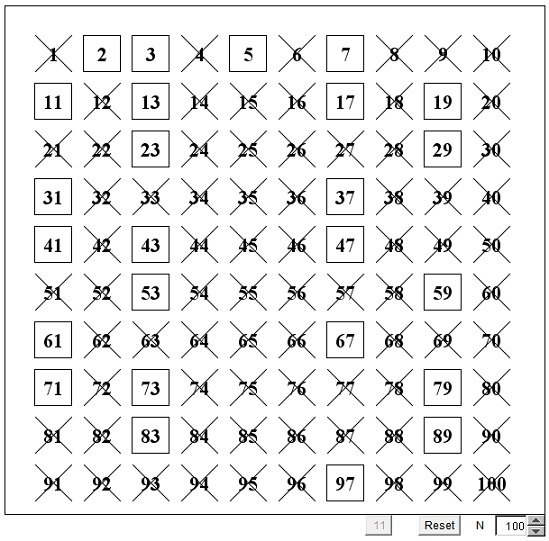
\includegraphics[width=0.50\textwidth]{sieve.jpg}
    \caption{Representation of the \sieve}
    \label{fig:tareador}
\end{figure}

\justify
We are given a sequential version of the program from which we will implement different parallel versions.


